\documentclass[12pt]{article}
\usepackage{fix-cm}
\usepackage{enumitem}
\usepackage{tikz}
\usetikzlibrary{trees, positioning, decorations.pathreplacing, calc}


% Define document-specific variables before loading template
\newcommand{\DocumentTitle}{Linguaggio Relazioni di Parentela}  % This will change for each

% Load the template
% header-template.tex
\usepackage{graphicx}
\usepackage{lastpage}
\usepackage{amssymb}
\usepackage{amsmath}
\usepackage{fancyhdr}
\usepackage{geometry}
\usepackage[colorlinks=true, linkcolor=blue, urlcolor=blue]{hyperref}
\usepackage{microtype}
% \usepackage{tgpagella}
%\usepackage[T1]{fontenc}
%\usepackage{newtxmath}

% Alternative font closer to University of Milan's official font
\usepackage[cmintegrals,cmbraces]{newtxmath}
\usepackage{ebgaramond-maths}
\usepackage[T1]{fontenc}

% Define default values for variables
\providecommand{\CourseTitle}{Introduzione al ragionamento scientifico}
\providecommand{\AcademicYear}{2024\mbox{-}25}
\providecommand{\Professor}{prof. Bernardino Sassoli de' Bianchi}
\providecommand{\DocumentDate}{Ottobre 2024}
\providecommand{\DocumentTitle}{Regole di inferenza}
\providecommand{\DocumentType}{Cheatsheet}

\geometry{a4paper, margin=1in}
\setlength{\headheight}{46.27916pt}
\addtolength{\topmargin}{-34.27916pt}



% Remove header rule
\renewcommand{\headrulewidth}{0pt}
\renewcommand{\footrulewidth}{0pt}

\fancypagestyle{firstpage}{%
    \fancyhf{} % clear all headers and footers
    \fancyhead[L]{%
        \begin{minipage}[c]{0.5\textwidth}
            
\includegraphics[width=3.5cm]{marchio-04.jpg}
        \end{minipage}%
    }
    \fancyhead[R]{%
        \begin{minipage}[c]{0.6\textwidth}
            \raggedleft
            {\footnotesize
            \CourseTitle\\
            \Professor\\
            A.A. \AcademicYear\\
            }
        \end{minipage}%
    }
}

% Define style for other pages
\fancypagestyle{followingpage}{%
    \fancyhf{} % clear all headers and footers
    \fancyhead[R]{\small\DocumentTitle}
    \fancyfoot[R]{\thepage}
}

% Set up the page styles to apply automatically
\AtBeginDocument{%
    \pagestyle{followingpage}% Set default style for all pages
    \thispagestyle{firstpage}% Override first page only
}

% Command for the standard title block
\newcommand{\MakeCustomTitle}[1]{%
    \begin{center}
    \vspace*{2cm}
    {\Large\textbf{#1}\\[0.5cm]
    \DocumentTitle}
    \end{center}
    \vspace{1cm}
}

\begin{document}

% Use the custom title command
\MakeCustomTitle{Esercitazioni di logica}

% Document content goes here

\section*{Esercizio 1}
\subsection*{Problema}
Il linguaggio delle relazioni di parentela $\mathcal{LRP}$ è costituito dalle seguenti relazioni primitive:
\begin{description}[labelindent=1cm, leftmargin=2cm]
   \item[Father (Padre):] $F(x, y)$ è vero se $x$ è il padre di $y$.
   \item[Mother (Madre):] $M(x, y)$ è vero se $x$ è la madre di $y$.
\end{description}
Dati i primitivi del linguaggio delle relazioni di parentela, definire le seguenti relazioni:
\begin{description}[labelindent=1cm, leftmargin=2cm]
   \item[Parent (Genitore):] $P(x, y)$ è vero se $x$ è il genitore di $y$.
   \item[Sibling (Fratello/Sorella):] $S(x, y)$ è vero se $x$ è fratello o sorella di $y$.
   \item[Grandfather (Nonno):] $G(x, y)$ è vero se $x$ è il nonno di $y$.
   \item[Cousin (Cugino/Cugina):] $C(x, y)$ è vero se $x$ è cugino o cugina di $y$.
   \item[Child (Figlio/Figlia):] $Ch(x, y)$ è vero se $x$ è il figlio o la figlia di $y$.
\end{description}

\subsection*{Soluzioni}
\begin{description}[
   align=left  % Aligns the descriptions to the left
]

   \item[Parent (Genitore):]
      $P(x, y) \equiv F(x, y) \lor M(x, y)$\footnotemark
      \footnotetext{$\equiv$ è usato come simbolo di equivalenza logica (anche "se e solo se").}

   \item[Sibling (Fratello/Sorella):]
      $
      S(x, y) \equiv x \neq y \land \exists z \left( P(z, x) \land P(z, y) \right)
      $

   \item[Grandfather (Nonno):]

      $
      F(x, y) \equiv \exists z \left(F(x, z) \land P(z, y) \right)
      $

   \item[Cousin (Cugina/Cugino):]
      $
      C(x, y) \equiv \exists z \exists w \left(P(z, x) \land P(w, y) \land S(z, w) \right)
      $

   \item [Child (Figlio/Figlia):]

   $
   Ch(x, y) \equiv F(y, x) \lor M(y, x)
   $
\end{description}
\section*{Esercizio 2}
\subsection*{Problema}
Aggiungiamo a $\mathcal{LRP}$ i due predicati primitivi:
\begin{description}[labelindent=1cm, leftmargin=2cm]
   \item[Maschio:] $\operatorname{male}(x)$ è vero se $x$ è di sesso maschile.
   \item[Femmina:] $\operatorname{female}(x)$ è vero se $x$ è di sesso femminile.
\end{description}
Definite le seguenti relazioni:
\begin{itemize}
   \item Figlia (Daughter)
   \item Figlio (Son)
   \item Fratello (Brother)
   \item Sorella  (Sister)
   \item Nipote maschio (Nephew)
   \item Zio (Uncle)
   \item Zia (Aunt)
   \item Nonno (Grandfather)
   \item Cugina/Cugino (Cousin)
\end{itemize}
\subsection*{Soluzioni}
\begin{description}[
   align=left          % Aligns the descriptions to the left
]
    \item[Daughter (Figlia):]
    \[
    \operatorname{daughter}(x, y) \equiv (\operatorname{father}(y, x) \lor \operatorname{mother}(y, x)) \land \operatorname{female}(x)
    \]

\item[Son (Figlio):]
   \[
   \operatorname{son}(x, y) \equiv (\operatorname{father}(y, x) \lor \operatorname{mother}(y, x)) \land \operatorname{male}(x)
   \]

\item[Brother (Fratello):]
   \[
   \operatorname{brother}(x, y) \equiv \operatorname{male}(x) \land \exists z \left( \operatorname{parent}(z, x) \land \operatorname{parent}(z, y) \right)
   \]

\item[Sister (Sorella):]
   \[
   \operatorname{sister}(x, y) \equiv
    \operatorname{female}(x) \land \exists z \left( \operatorname{parent}(z, x) \land \operatorname{parent}(z, y) \right)
   \]
   \begin{center}
      \begin{tikzpicture}[
         node distance=2.5cm,
         relation/.style={font=\footnotesize\itshape, teal},
         operator/.style={circle, draw, minimum size=0.5cm},
         male/.style={operator, draw=blue},
         female/.style={operator, draw=red},
         legend/.style={font=\footnotesize, align=left}
      ]
         % Nodes for operators
         \node[operator] (z) {$z$};
         \node[operator] (y) [below right of=z] {$y$};
         \node[female] (x) [below left of=z] {$x$};

         % Arrows with labels in different style
         \draw[->] (z) -- node[above right, relation] {parent} (y);
         \draw[->] (z) -- node[above left, relation] {parent} (x);

         % Legend
         \node[legend, below right=0.5cm and -1cm of x] {
            \tikz\node[female,scale=0.4] {}; = female
         };

      \end{tikzpicture}
   \end{center}

\item[Nephew (Nipote maschio):]
   \[
   \operatorname{nephew}(x, y) \equiv \operatorname{male}(x) \land \exists z \left( \operatorname{sibling}(z, y) \land (\operatorname{father}(z, x) \lor \operatorname{mother}(z, x)) \right)
   \]
   \begin{center}
      \begin{tikzpicture}[
         node distance=2.5cm,
         relation/.style={font=\footnotesize\itshape, teal},
         operator/.style={circle, draw, minimum size=0.5cm},
         male/.style={operator, draw=blue},
         legend/.style={font=\footnotesize, align=left}
      ]
         % Nodes for operators
         \node[operator] (z) {$z$};
         \node[operator] (y) [right of=z] {$y$};
         \node[male] (x) [below right of=y] {$x$};

         % Arrows with labels in different style
         \draw[<->] (z) -- node[above, relation] {sibling} (y);
         \draw[->] (y) -- node[right, relation] {parent} (x);

         % Legend
         \node[legend, below right=0.5cm and -1cm of x] {
            \tikz\node[male,scale=0.4] {}; = male
         };

      \end{tikzpicture}
   \end{center}
\item[Uncle (Zio):]
   \[
   \operatorname{uncle}(x, y) \equiv \operatorname{male}(x) \land \exists z \left( \operatorname{parent}(z, y) \land \operatorname{sibling}(x, z) \right)
   \]
   \begin{center}
      \begin{tikzpicture}[
         node distance=2.5cm,
         relation/.style={font=\footnotesize\itshape, teal},
         operator/.style={circle, draw, minimum size=0.5cm},
         male/.style={operator, draw=blue},
         legend/.style={font=\footnotesize, align=left}
      ]
         % Nodes for operators
         \node[male] (x) {$x$};
         \node[operator] (z) [right of=x] {$z$};
         \node[operator] (y) [below right of=z] {$y$};

         % Arrows with labels in different style
         \draw[<->] (x) -- node[above, relation] {sibling} (z);
         \draw[->] (z) -- node[right, relation] {parent} (y);

         % Legend
         \node[legend, below right=0.5cm and -1cm of y] {
            \tikz\node[male,scale=0.4] {}; = male
         };
      \end{tikzpicture}
   \end{center}
\item[Aunt (Zia):]
   \[
   \operatorname{aunt}(x, y) \equiv \operatorname{female}(x) \land \exists z \left( \operatorname{parent}(z, y) \land \operatorname{sibling}(x, z) \right)
   \]
   \begin{center}
      \begin{tikzpicture}[
         node distance=2.5cm,
         relation/.style={font=\footnotesize\itshape, teal},
         operator/.style={circle, draw, minimum size=0.5cm},
         male/.style={operator, draw=blue},
         female/.style={operator, draw=red},
         legend/.style={font=\footnotesize, align=left}
      ]
         % Nodes for operators
         \node[female] (x) {$x$};
         \node[operator] (z) [right of=x] {$z$};
         \node[operator] (y) [below right of=z] {$y$};

         % Arrows with labels in different style
         \draw[<->] (x) -- node[above, relation] {sibling} (z);
         \draw[->] (z) -- node[right, relation] {parent} (y);

         % Legend
         \node[legend, below right=0.5cm and -1cm of y] {
            \tikz\node[female,scale=0.4] {}; = female
         };
      \end{tikzpicture}
   \end{center}
\item[Grandfather (Nonno):]
    \[
    \operatorname{grandfather}(x, y) \equiv \operatorname{male}(x) \land \exists z \left( \operatorname{parent}(x, z) \land \operatorname{parent}(z, y) \right)
    \]
    \begin{center}
      \begin{tikzpicture}[
         node distance=2.5cm,
         relation/.style={font=\footnotesize\itshape, teal},
         operator/.style={circle, draw, minimum size=0.5cm},
         male/.style={operator, draw=blue},
         female/.style={operator, draw=red},
         legend/.style={font=\footnotesize, align=left}
      ]
         % Nodes for operators
         \node[male] (x) {$x$};
         \node[operator] (z) [below of=x] {$z$};
         \node[operator] (y) [below of=z] {$z$};

         % Arrows with labels in different style
         \draw[->] (x) -- node[midway, left, relation] {parent} (z);
         \draw[->] (z) -- node[midway, left, relation] {parent} (y);

         % Legend
         \node[legend, below right=0.5cm and -1cm of y] {
            \tikz\node[male,scale=0.4] {}; = male
         };
      \end{tikzpicture}
   \end{center}
\item[Cousin (Cugino/Cugina):]
    \[
    \operatorname{cousin}(x, y) \equiv \exists z \exists w \left( \operatorname{parent}(z, x) \land \operatorname{parent}(w, y) \land \operatorname{sibling}(z, w) \right)
    \]
    \begin{center}
      \begin{tikzpicture}[
         node distance=2.5cm,
         relation/.style={font=\footnotesize\itshape, teal},
         operator/.style={circle, draw, minimum size=0.5cm},
         male/.style={operator, draw=blue},
         female/.style={operator, draw=red},
         legend/.style={font=\footnotesize, align=left}
      ]
         % Nodes for operators
         \node[operator] (z) {$z$};
         \node[operator] (w) [right of=z] {$w$};
         \node[operator] (x) [below of=z] {$x$};
         \node[operator] (y) [below of=w] {$y$};

         % Arrows with labels in different style
         \draw[<->] (z) -- node[midway, above, yshift=2pt, relation] {sibling} (w);
         \draw[->] (z) -- node[midway, left, relation] {parent} (x);
         \draw[->] (w) -- node[midway, right, relation] {parent} (y);

        ;
      \end{tikzpicture}
   \end{center}
\end{description}
\section*{Esercizio 3}
\subsection*{Problema}
Definite termini neutri (come «sibling», «parent» e «child» nell’esercizio precedente) per «nephew-niece» e «uncle-aunt».
\subsection*{Soluzioni}
\begin{description}[
   align=left          % Aligns the descriptions to the left
]
    \item[Nibling (Zio/Zia):]
    \[
      \operatorname{Nibling}(x, y) \equiv \exists z\operatorname{parent}(z, x) \land \operatorname{sibling}(z, y)
        \]
    \begin{center}
      \begin{tikzpicture}[
         node distance=2.5cm,
         relation/.style={font=\footnotesize\itshape, teal},
         operator/.style={circle, draw, minimum size=0.5cm},
         male/.style={operator, draw=blue},
         female/.style={operator, draw=red},
         legend/.style={font=\footnotesize, align=left}
      ]
         % Nodes for operators
         \node[operator] (y) {$y$};
         \node[operator] (z) [right of=y] {$z$};
         \node[operator] (x) [below of=z] {$x$};

         % Arrows with labels in different style
         \draw[<->] (z) -- node[midway, above, yshift=2pt, relation] {sibling} (y);
         \draw[->] (z) -- node[midway, left, relation] {parent} (x);
        ;
      \end{tikzpicture}
   \end{center}

      \item[Pibling (Nipote):]
    \[
    \operatorname{Pibling}(x, y) \equiv \exists z\operatorname{parent}(z, y) \land \operatorname{sibling}(x, z)
      \]
      \begin{center}
      \begin{tikzpicture}[
         node distance=2.5cm,
         relation/.style={font=\footnotesize\itshape, teal},
         operator/.style={circle, draw, minimum size=0.5cm},
         male/.style={operator, draw=blue},
         female/.style={operator, draw=red},
         legend/.style={font=\footnotesize, align=left}
      ]
         % Nodes for operators
         \node[operator] (x) {$x$};
         \node[operator] (z) [right of=y] {$z$};
         \node[operator] (y) [below of=z] {$y$};

         % Arrows with labels in different style
         \draw[<->] (z) -- node[midway, above, yshift=2pt, relation] {sibling} (x);
         \draw[->] (z) -- node[midway, left, relation] {parent} (y);
        ;
      \end{tikzpicture}
   \end{center}
\end{description}
\end{document}